%
% Chapter 3
%
\chapter{Requirements}\label{chap:requirements}

To meet the objectives of the SCAR project, the application to be developed, named DiGo Certify, should allow different stakeholders to access, share, and issue certificates on the Ethereum blockchain from anywhere in the world, offering a futuristic solution to the problems described in section (...).

The DiGo Certify application aims to address the needs of various stakeholders in the educational ecosystem. Mandatory and optional requirements have been defined based on essential functionalities and additional enhancements desired for the application.

.



\section{Stakeholders}\label{subsec:stakeholders}
The SCAR solution involves three main stakeholders: students or alumni, employers or third-party entities, and college administrators. Each plays a crucial role in the application's ecosystem.

\subsubsection{Role of Each Stakeholder and Actions They Can Perform:}

\begin{itemize}

    \item \textbf{Students or Alumni:} Students or alumni are the essence of our application. They will have the ability to register on the mobile application, where they can securely upload and store their academic certificates on the blockchain. Additionally, students or alumni can view and share their certificates with employers or third-party entities during recruitment processes, providing a transparent and efficient experience.

    \item \textbf{College Administrators:} College administrators are responsible for issuing and validating academic certificates provided by the educational institution. They will have access to the application to issue and authenticate certificates for students or alumni, thereby ensuring the integrity and validity of the documents.

    \item \textbf{Employers or External Entities:} Employers play a crucial role in requesting the verification of academic certificates during job interviews. By accessing the DiGo Certify platform, employers or external entities can instantly verify the authenticity of the certificates presented by students or alumni, without the need of possessing a wallet and with this ensuring a more reliable and transparent recruitment process.

\end{itemize}

\section{Mandatory Requirements:}

\begin{itemize}

    \item \textbf{Implementation of the mobile application using React Native with Expo platform:} The choice of React Native along with the Expo platform provides an effective approach for developing multiplatform mobile applications. This ensures a consistent experience for users, regardless of the device used, and facilitates the development process for the development team.

    \item \textbf{Utilization of smart contracts in Solidity to store and validate academic certificates on the Ethereum blockchain:} The use of smart contracts in Solidity offers a secure and reliable solution for storing and validating academic certificates on the Ethereum blockchain. This approach ensures data integrity and immutability, making the DiGo Certify platform highly reliable and resistant to fraud.

    \item \textbf{Development of features for registration, authentication, and secure storage of certificates on the blockchain:} Developing robust features for registering, authenticating, and securely storing certificates on the blockchain is essential to ensure the security and reliability of the DiGo Certify platform. These features should be designed with a focus on usability and security, providing an intuitive and transparent experience for users.

\end{itemize}

\subsection{Optional Requirements:}

\begin{itemize}

    \item \textbf{Integration of additional features, such as real-time notifications and sharing of certificates through digital channels:} Incorporating extra functionalities like real-time notifications and certificate sharing through digital channels, such as social media platforms, can further enhance the user experience on the DiGo Certify platform. This enhancement can boost usability and attract new users to the platform.

\end{itemize}

\section{Use Cases}\label{sec:use-cases}

The following use cases describe the interactions between the different stakeholders in the DiGo Certify platform. Each use case outlines the actions performed by the stakeholders and the expected outcomes of these interactions. The use cases are illustrated using diagrams based on the 4+1 View Model, which provides a comprehensive view of the system from multiple perspectives\cite{4+1-architecture-viewmodel}.

\subsection{Use Case 1: Student Registration and Certificate Requesting}

\begin{figure}[H]
    \centering
    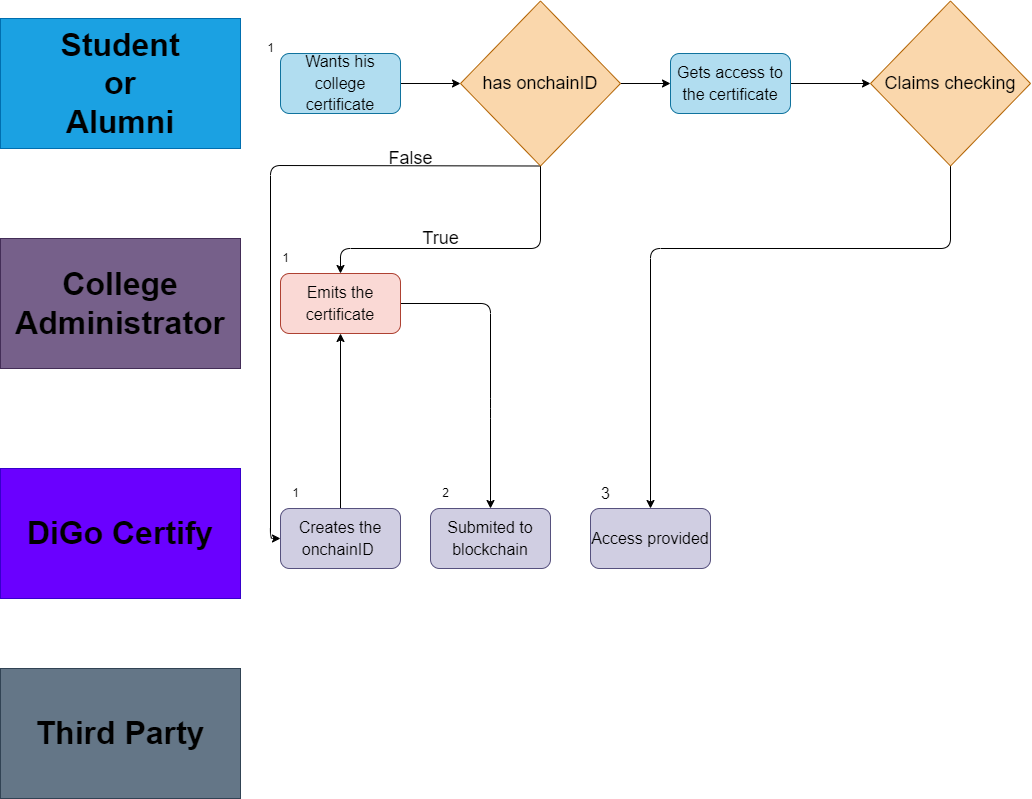
\includegraphics[width=0.6\textwidth, height=0.6\textheight, keepaspectratio]{./assets/certificate-requesting.drawio.png}
    \caption{Use Case 1: Student Registration and Certificate Requesting.}
    \label{fig:use-case-1}
\end{figure}

\begin{itemize}

    \item \textbf{Actors:} Student, College Administrator
    \item \textbf{Description:} A student registers on the mobile application and requests academic certificates from the college administrator.
    \item \textbf{Preconditions:} The student has access to the DiGo Certify platform. The college administrator has access to the platform and the student's academic records.
    \item \textbf{Postconditions:} The student receives the academic certificates and stores them on the blockchain.
    \item \textbf{Main Flow:}
    \item 1. The student downloads the \texttt{DiGo Certify} mobile application from the app store.
    \item 2. The student registers himself using their email address and connecting a wallet to the application.
    \item 3. The student requests academic certificates from the college administrator.
    \item 4. The college administrator issues the certificates, submitting them to the blockchain and
          emits the claims that will allow the student to access the certificates.
    \item 5. The student receives a notification that the certificates are available for download.
    \item \textbf{Alternative Flow:}
    \item 1.1 The student already has an account on the DiGo Certify platform.
    \item 1.2 The student logs in to their account using their email address.
    \item 1.3 The student requests additional academic certificates from the college administrator.
    \item 1.4 The college administrator issues the new certificates and submits them to the blockchain.
    \item 1.5 The student receives a notification that the certificates are available for download.
    \item \textbf{Exceptions:}
    \item 1. The student enters an invalid email address during registration.
    \item 2. The student fails to register on the application due to an error in the process.
    \item 3. The college administrator does not issue the certificates to the student.
    \item \textbf{Notes:} This use case illustrates the process of student registration and certificate requesting on the mobile application. It emphasizes the importance of secure and transparent interactions between the student and the college administrator, enabled by the blockchain technology.
\end{itemize}

\subsection{Use Case 2: Certificate Validation by an External Entity}

\begin{figure}[H]
    \centering
    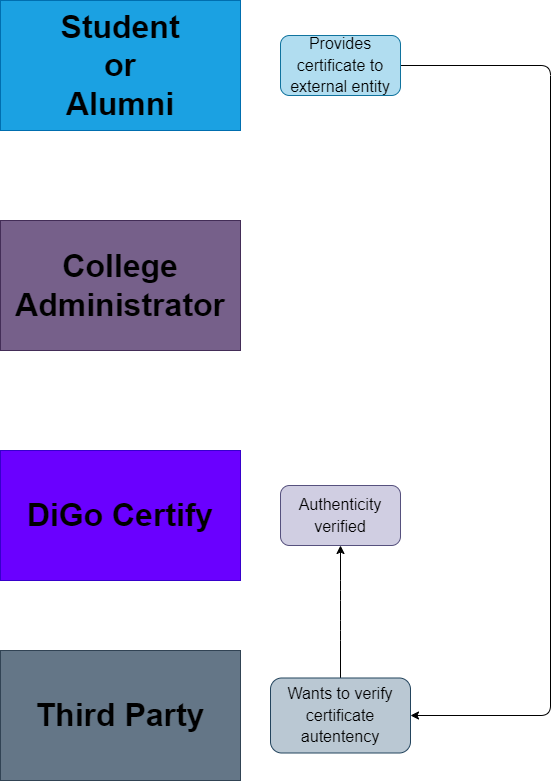
\includegraphics[height=0.6\textwidth, keepaspectratio]{./assets/certificate-validation.drawio.png}
    \caption{Use Case 2: Certificate Verification by an External Entity.}
    \label{fig:use-case-2}
\end{figure}

\begin{itemize}

    \item \textbf{Actors:} External Entity, Student
    \item \textbf{Description:} For the purpose of a job application, an external entity verifies the authenticity of the student's academic certificates on the mobile application.
    \item \textbf{Preconditions:} The employer has access to the \texttt{DiGo Certify} application. The student has shared their certificates with the employer.
    \item \textbf{Postconditions:} The employer confirms the authenticity of the student's certificates and proceeds with the recruitment process.
    \item \textbf{Main Flow:}
    \item 1. The employer does not need to have a wallet to access the application.
    \item 2. The employer scans the QR code or accesses the link shared by the student to view the certificates.
    \item 3. The employer views the student's certificates and verifies their authenticity on the blockchain.
    \item 4. The employer confirms the authenticity of the certificates and proceeds with the recruitment process.
    \item \textbf{Exceptions:}
    \item 1. The employer fails to verify the authenticity of the certificates due to an error in the process.
    \item 2. The employer does not confirm the authenticity of the certificates.
    \item \textbf{Notes:} This use case illustrates the process of certificate verification by an employer on the \texttt{DiGo Certify} mobile application. It emphasizes the importance of transparency and trust in the recruitment process, enabled by the blockchain technology.

\end{itemize}

\subsection{Use Case 3: Student or Alumni requests a change to the certificate}

\begin{figure}[H]
    \centering
    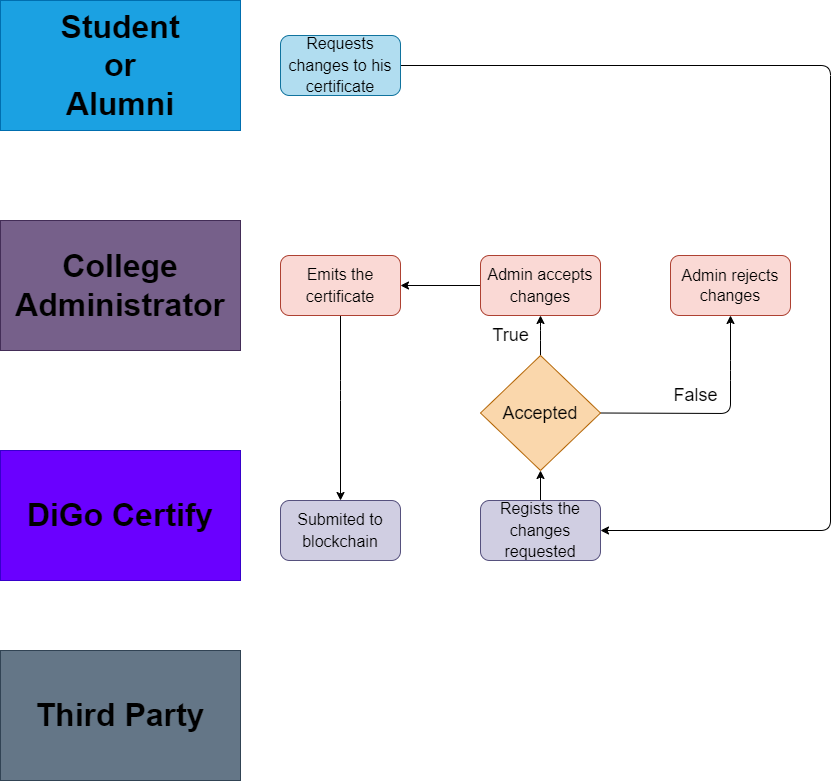
\includegraphics[width=0.6\textwidth, height=0.6\textheight, keepaspectratio]{./assets/certificate-update.drawio.png}
    \caption{Use Case 3: Student or Alumni requests a change to the certificate.}
    \label{fig:use-case-3}
\end{figure}

\begin{itemize}

    \item \textbf{Actors:} Student, College Administrator
    \item \textbf{Description:} A student or alumni requests a change to the academic certificates issued by the college administrator.
    \item \textbf{Preconditions:} The student has access to the DiGo Certify platform. The college administrator has access to the platform and the student's academic records.
    \item \textbf{Postconditions:} The student receives the updated academic certificates and stores them on the blockchain.
    \item \textbf{Main Flow:}
    \item 1. The student logs in to the \texttt{DiGo Certify} mobile application.
    \item 2. The student requests a change to the academic certificates from the college administrator.
    \item 3. The college administrator updates the certificates, submitting them to the blockchain and emits the claims that will allow the student to access the updated certificates.
    \item 4. The student receives a notification that the updated certificates are available for download.
    \item \textbf{Exceptions:}
    \item 1. The student fails to log in to the application due to an error in the process.
    \item 2. The student does not request a change to the academic certificates.
    \item 3. The college administrator does not update the certificates for the student.
    \item \textbf{Notes:} This use case illustrates the process of requesting a change to academic certificates on the mobile application. It emphasizes the importance of maintaining accurate and up-to-date records on the blockchain, enabled by the blockchain technology.

\end{itemize}